
\documentclass[oneside]{diretrizes}            % Imprimir apenas frente
%\documentclass[doubleside]{diretrizes}        % Imprimir frente e verso

% Importações de pacotes
\usepackage[alf, abnt-emphasize=bf, recuo=0cm, abnt-etal-cite=2, abnt-etal-list=0]{abntex2cite}  % Citações padrão ABNT
\usepackage[utf8]{inputenc}                         % Acentuação direta
\usepackage[T1]{fontenc}                            % Codificação da fonte em 8 bits
\usepackage{graphicx}                               % Inserir figuras
\usepackage{amsfonts, amssymb, amsmath}             % Fonte e símbolos matemáticos
\usepackage{booktabs}                               % Comandos para tabelas
\usepackage{verbatim}                               % Texto é interpretado como escrito no documento
\usepackage{multirow, array}                        % Múltiplas linhas e colunas em tabelas
\usepackage{indentfirst}                            % Endenta o primeiro parágrafo de cada seção.
\usepackage{microtype}                              % Para melhorias de justificação?
\usepackage[algoruled, portuguese]{algorithm2e}     % Escrever algoritmos
\usepackage{float}                                  % Utilizado para criação de floats
\usepackage{times}                                  % Usa a fonte Times
\usepackage{nomencl}

% Inclui o preâmbulo do documento
%
% Documento: Preâmbulo
%

\instituicao{INSTITUTO FEDERAL DE EDUCAÇÃO, CIÊNCIA E\\
TECNOLOGIA FLUMINENSE \textit{CAMPUS }ITAPERUNA}
\abreviatura{IFF}
\departamento{}
\local{ITAPERUNA}
\programa{BACHARELADO EM SISTEMAS DE INFORMAÇÃO}
\nomeautor{WILLIAN CAMACHO LOPES}
\titulotb{REVISAPP - SOFTWARE PARA GARANTIA E QUALIDADE}
%\subtitulo{Subtítulo do trabalho}
\data{2019}
\grau{Tecnólogo}
\dataapresentacao{DD/MM/20AA}

%Dados Orientador
\orientador{Ford Perfect}
\coorientador{Anderson Black}
\instOrientador{IFRS}
\departamentoorientador{Campus Restinga}
\titulacaoorientador{Prof. Me.}

%Dados Coorientador
\coorientador{Artur Dent}
\instCoorientador{IFRS}
\departamentocoorientador{Campus Restinga}
\titulacaocoorientador{Prof. Dr.}

%Dados Examinador 1
\nmexamum{Mestre dos Magos}
\instexamum{IFRS}
\departamentoexamum{Campus Restinga}
\titulacaoexamum{Prof.}

%Dados Examinador 2
\nomeexamdois{Mestre Splinter}
\instexamdois{IFRS}
\departamentoexamdois{Campus Restinga}
\titulacaoexamdois{Prof. Me.}


% Define as cores dos links e informações do PDF
\makeatletter
\hypersetup{
    portuguese,
    colorlinks,
    linkcolor=black,
    citecolor=black,
    filecolor=black,
    urlcolor=black,
    breaklinks=true,
    pdftitle={\@title},
    pdfauthor={\@author},
    pdfsubject={\imprimirpreambulo},
    pdfkeywords={abnt, latex, abntex, abntex2}
}
\makeatother

% Redefinição de labels
\renewcommand{\algorithmautorefname}{Algoritmo}
\def\equationautorefname~#1\null{Equa\c c\~ao~(#1)\null}

% Cria o índice remissivo
\makeindex

% Início do documento
\begin{document}

    % Retira espaço extra obsoleto entre as frases.
    \frenchspacing

    % Elementos pré textuais
    \pretextual
    %
% Documento: Capa
%

\makeatletter
\begin{capa}
	\thispagestyle{empty}%limpa estilo da pagina
	\setlength{\baselineskip}{0.72\baselineskip}
    \begin{center} %Alinhamento centralizado
	

    \textbf{\expandafter\uppercase\expandafter{\imprimirinstituicao}}\\
    \textbf{\expandafter\uppercase\expandafter{\imprimirdepartamento}}\\
    \textbf{\expandafter\uppercase\expandafter{\imprimirprograma}}\\
	\vspace*{5cm}%Espaçamento entre linhas
	\small\textbf{\expandafter\uppercase\expandafter{\imprimirnomeautor}}\\
	\vspace*{6cm}%Espaçamento entre linhas	
	\small\textbf{\expandafter\uppercase\expandafter{\imprimirtitulotb}}\\
	\vspace*{9.5cm}%%Espaçamento entre linhas
	\small\textbf{\expandafter\uppercase\expandafter{\imprimirlocal}}\\
	\small\textbf{\expandafter\uppercase\expandafter{\imprimirdata}}\\
		
		
		
	\end{center} %Alinhamento centralizado
\end{capa}
\makeatother

	

              % Capa
    %
% Documento: FOLHA DE ROSTO
%

\makeatletter
\begin{folhaderosto}
	\thispagestyle{empty}%limpa estilo da pagina
	
    \begin{center}
    
		\small\textbf{\expandafter\uppercase\expandafter{\imprimirnomeautor}}\\
		\vspace*{8.2 cm}%Espaço entre linhas
		\normalsize\textbf{\expandafter\uppercase\expandafter{\imprimirtitulotb}}\\
		
    \end{center}
	
	\vspace*{0.35 cm}%Espaçamento entre linhas
		    \large%tamanho da fonte 
    		\hfill%Estica horizontamente  com espaços
	    	\begin{minipage}{8 cm}%Minipagina
	    		\begin{small} %Muda tamanho da fonte
	    		\setlength{\baselineskip}{0.7\baselineskip}
				
		    	{Trabalho de Conclusão de Curso apresentada como requisito parcial para obtenção do grau de
		    	{\imprimirgrau } em {\imprimirprograma } da {\imprimirinstituicao}{ - }{\imprimirabreviatura},
		    	{\imprimirdepartamento}.}\\{
		    	}\\Orientador: {\imprimirtitulacaoorientador }{ }{\imprimirorientador}\\{
		    	}\\Co-orientador: {\imprimirtitulacaocoorientador }{ }{\imprimircoorientador}
				
				
				\end{small} %Muda tamanho da fonte
		    \end{minipage}%%Minipagina
		    	
		    \vspace*{10 cm}%Espaçamento entre linhas
		    
		    \begin{center} %Alinhamento centralizado
		    	\normalsize %Muda tamanho da fonte
	    		\imprimirlocal\\
	    		\imprimirdata
	    	\end{center}%Alinhamento centralizado

\end{folhaderosto}
\makeatother
        % Folha de rosto
    %
% Documento: FOLHA APROVAÇÃO
%

\makeatletter
\begin{folhadeaprovacao}

\thispagestyle{empty}%limpa estilo da pagina
	
	\begin{center}
    
		\small\textbf{\expandafter\uppercase\expandafter{\imprimirnomeautor}}\\
		\vspace*{3.0 cm}%Espaço entre linhas
		\normalsize\textbf{\expandafter\uppercase\expandafter{\imprimirtitulotb}}
		
    \end{center}
	
	\vspace*{0.35 cm}%Espaçamento entre linhas
		    \large%tamanho da fonte 
    		\hfill%Estica horizontamente  com espaços
	    	\begin{minipage}{8 cm}%Minipagina
	    		\begin{small} %Muda tamanho da fonte
	    		\setlength{\baselineskip}{0.7\baselineskip}
				
		    	{Trabalho de Conclusão de Curso apresentado como requisito parcial para obtenção do grau de
		    	{\imprimirgrau } em {\imprimirprograma } do {\imprimirinstituicao}{ - }{\imprimirabreviatura},
		    	{\imprimirdepartamento}.}\\{
		    	}\\				
				
				\end{small} %Muda tamanho da fonte
		    \end{minipage}%%Minipagina
		    	
		    \vspace*{0.6 cm}%Espaçamento entre linhas
		    
		    \large%%tamanho da fonte 
    		\hfill%%Estica horizontamente  com espaços
	    	 
		    
		    \normalsize %Muda tamanho da fonte
		    \vspace*{1.5 cm}%Espaçamento entre linhas
		    
		    \begin{minipage}{9 cm }%%Minipagina
		    {Data de Aprovação: {\imprimirdataapresentacao}}\\
		    \end{minipage}%Minipagina
			
			\begin{center}%Alinhamento centralizado
		    	\vspace*{1.21 cm}%Espaçamento entre linhas
				\textbf{Banca Examinadora}\\ %Negrito
						
				\vspace*{1 cm}%Espaçamento entre linhas
				\rule{9 cm}{.1 mm}\\
				{\imprimirtitulacaoorientador}{ }{\imprimirorientador} - {\imprimirinstOrientador} - {\imprimirdepartamentoorientador}\\
				
				Orientador\\
				
				\vspace*{1 cm}%Espaçamento entre linhas
				\rule{9 cm}{.1 mm}\\
				{\imprimirtitulacaocoorientador}{ }{\imprimircoorientador} - {\imprimirinstCoorientador} - {\imprimirdepartamentocoorientador}\\
				
				Co-Orientador\\
			
				\vspace*{1 cm}%Espaçamento entre linhas
				\rule{9 cm}{.1 mm}\\
				\imprimirtitulacaoexamum{ }\imprimirnmexamum - \imprimirinstexamum - \imprimirdepartamentoexamum\\
				Membro da Banca
				
				\vspace*{1 cm}%Espaçamento entre linhas
				\rule{9 cm}{.1 mm}\\				
								
				\imprimirtitulacaoexamdois{ }\imprimirnomeexamdois - \imprimirinstexamdois - \imprimirdepartamentoexamdois\\
				Membro da Banca
				\vspace*{1.3 cm}%Espaçamento entre linhas
		    \end{center}%Alinhamento centralizado


\end{folhadeaprovacao}
\makeatother
    % Folha de aprovação
    %
% Documento: Folha Catalográfica
%

\thispagestyle{empty}
\vspace*{\fill}

 \begin{flushleft}
\small \setlength{\baselineskip}{0.8\baselineskip}INSTITUTO FEDERAL DE EDUCAÇÃO, CIÊNCIA E TECNOLOGIA DO RIO GRANDE DO SUL\\
Reitor: Prof. Osvaldo Casares Pinto\\
Pró-Reitora de Ensino: Profa. Clarice Monteiro Escott\\
Diretor do Campus Restinga: Prof. Gleison Samuel do Nascimento\\
Coordenador do Curso de Ciência da Computação: Prof. Rafael Pereira Esteves\\
Bibliotecária-Chefe do Campus Restinga: Paula Porto Pedone\\
\end{flushleft}



    %
% Documento: Dedicatória
%

\thispagestyle{empty}
\begin{dedicatoria}

Aqui você pode inserir uma homenagem ou dedica seu trabalho.



\end{dedicatoria}
       % Dedicatória
    %
% Documento: Agradecimento
%

\begin{agradecimento}

Neste trecho você faz agradecimentos dirigidos aqueles que contribuíram de maneira relevante a elaboração do trabalho. Elemento opcional segundo a norma da ABNT NBR 14724 de 2011.

\end{agradecimento}

    % Agradecimentos
    %
% Documento: Epígrafe
%
\thispagestyle{empty}
\begin{epigrafe}


O fator decisivo para vencer o maior obstáculo é, invariavelmente, ultrapassar o obstáculo anterior.{\\}{\\}

\begin{autorepigrafe}
Henry Ford
\end{autorepigrafe}

\end{epigrafe}


          % Epígrafe
    %
% Documento: Resumo (Português)
%

\begin{RESUMO}
\thispagestyle{empty}
	\begin{SingleSpace}
	
		\hspace{-1.2 cm}Conforme as normas NBR 14724:2011 da ABNT, o resumo é elemento obrigatório, constituído de uma sequência de frases concisas e objetivas e não de uma simples enumeração de tópicos, não ultrapassando 500 palavras, seguido, logo abaixo, das palavras representativas do conteúdo do trabalho, isto é, palavras-chave e/ou descritores.

		\vspace*{0.5cm}\hspace{-1.3 cm}\textbf{Palavras-chave}: Conclusão. Trabalho. Curso. NBR. ABNT.
		
		
		
	\end{SingleSpace}
\end{RESUMO}


          % Resumo na língua vernácula
    %
% Documento: Resumo (Inglês)
%

\begin{ABSTRACT}
	\begin{SingleSpace}
	
		\hspace{-1.3 cm}Versão em língua estrangeira do resumo. Obrigatório, pela ABNT. O título é ABSTRACT, em inglês, RESUMEN, em espanhol castelhano, e RÉSUMÉ, em francês.

		\vspace*{0.5cm}\hspace{-1.3 cm}\textbf{Keywords}: Work. Course. NBR. ABNT.
		
		
	\end{SingleSpace}

\end{ABSTRACT}
          % Resumo em língua estrangeira
    %
% Documento: Lista de figuras
%

\pdfbookmark[0]{\listfigurename}{lof}
\listoffigures*
\cleardoublepage

      % Lista de figuras
    %
% Documento: Lista de tabelas
%

\pdfbookmark[0]{\listtablename}{lot}
\listoftables*
\cleardoublepage
      % Lista de tabelas
    %
% Documento: Lista de quadros
%

\pdfbookmark[0]{\listofquadrosname}{loq}
\listofquadros*
\cleardoublepage
      % Lista de quadros
    %
% Documento: Lista de abreviaturas e siglas
%

\begin{siglas}
	\setlength{\baselineskip}{0.7\baselineskip}
	
    \item[ABNT] Associação Brasileira de Normas Técnicas
    \item[TCC] Trabalho de Conclusão do Curso
    \item[NBR] Norma Brasileira
    \item[AI] \textit{Artificial Intelligency}
    
\end{siglas}


       % Lista de abreviaturas e siglas
    %%
% Documento: Lista de símbolos
%

\begin{simbolos}
    \item[$ \Gamma $] Letra grega Gama
    \item[$ \lambda $] Comprimento de ondada
    \item[$ \in $] Pertence
\end{simbolos}
     % Lista de símbolos
    \sumario

    % Elementos textuais
    \textual
    %
% Documento: Introdução
%

\chapter{INTRODUÇÃO}\label{chap:introducao}



\section{Justificativa}

\section{Objetivos}

\subsection{Objetivos Gerais}

O objetivo é o desenvolvimento de um software, com uma interface simples e visual, para ajudar engenheiros de software, analistas de sistemas e equipes de garantia e testes de software a descobrir e documentar erros de função, lógica ou implementação em programas, assegurando a qualidade do software e garantindo que ele atenda aos requisitos e às regras predefinidas.

\subsection{Objetivos Específicos}

\begin{itemize}
    \item Manter o registro de todas as reuniões realizadas;
    \item Manter uma base de dados para consultas (reuniões e atas);
    \item Automatizar/informatizar o registo das reuniões;
    \item Agilizar em até 30\% o registro das reuniões/atas;
    \item Facilitar o apontamento das melhorias ao produto;
    \item Garantir consistência do software à medida que mudanças ocorram;
\end{itemize}
            % Introdução
    %
% Documento: Disposições
%

\chapter{REFERENCIAL TEÓRICO}\label{chap:referencial}

Neste capítulo iremos entender os conceitos de qualidade e qualidade de \textit{software}; veremos os ciclos de desenvolvimento de um \textit{software} e a importância de escolher um ciclo adequado; e, como funciona a técnica - que norteará o desenvolvimento do \textit{software} proposto neste trabalho - de garantia e qualidade qualidade RTF - Revisão Técnica Formal.

\section{Qualidade}


Qualidade, na definição do dicionário Michaelis \footnote{https://michaelis.uol.com.br/moderno-portugues/busca/portugues-brasileiro/qualidade/}, significa "atributo, condição natural ou propriedade pela qual algo ou alguém se individualiza, distinguindo-se dos demais". Derivada do latin \textit{qualitate}, a palavra também pode expressar "precisão, o grau de perfeição ou conformidade a certo padrão". Em suma, como corrobora o Dicionário Aurélio\footnote{https://dicionariodoaurelio.com/qualidade}, "é a maneira de ser de algo ou alguém, sua superioridade ou excelência".

No decorrer da história, vários autores tentaram definir o real significado de qualidade. Para \citeonline{GARVIN2002}, esse termo dispõe de várias interpretações e por isso "é essencial um melhor entendimento do termo para que a qualidade possa assumir um papel estratégico". Muitos procuraram defini-lá de acordo com seus diversos pontos de vista. Na visão generalista de Philip Crosby, qualidade é apenas atendimento aos requisitos. Ele defende a ideia de que não se deve preocupar com percepções subjetivas de qualidade, e sim focar-se no atendimento aos requisitos e especificações do produto \cite{CROSBY1979}.

Para \citeonline{CAMPOS1992}, qualidade é a adequação ao uso, é a totalidade das características de um produto ou serviço que se relacionam com sua capacidade de atender às necessidades de um cliente. Qualidade é o grau no qual um conjunto de características inerentes satisfaz aos requisitos. \cite{ISO90002005}

\begin{citacao}

A maioria das pessoas concorda que qualidade é aquilo que produz satisfação, que está relacionada a um preço justo, a um produto que funciona corretamente e a um serviço prestado de forma a superar as expectativas de quem dela faz uso. \cite[p. 52]{VERGUEIRO2002} 

\end{citacao}

Na relação entre qualidade, produto e cliente final, \citeonline{DEMING1986} sustenta que qualidade de um produto é definida por meio da percepção do cliente final daquele produto, portanto, por mais que um produto possa atender a todos os requisitos técnicos e ser vendido por um preço justo, se não for valorizado pelo cliente, não tem qualidade.

A defesa de \citeonline{ARAUJO2007} é que a qualidade é busca pela perfeição, almejando agradar aos clientes que estão cada vez mais exigentes. "Qualidade é adequação ao uso, é aquilo que não cria problemas, é fazer a coisa certa na primeira vez." \cite[p. 15]{RANGEL1195}

Assim como existem diversos conceitos, a qualidade possui também inúmeros objetivo. Esses objetivos estendem-se ao produto: (variáveis e atributos que podem ser medidos e controlados); ao usuário: (produto é o que o cliente compra); à fabricação: (adequação às normas e às especificações); ao valor: (adequado ao uso e ao preço). \cite{MARTINSELAUGENI2006}



%objetivo da qualidade

%padrões e normas para garantir a qualidade

\section{Qualidade de Software}

\citeonline{PRESSMAN2002} define qualidade de \textit{software} como a conformidade com os requisitos; com os padrões de desenvolvimento e com as características implícitas que são esperadas em todo \textit{software} desenvolvido profissionalmente. 
 
 A definição de Alexandre Bartié vai de encontro ao de Pressaman: "[...] qualidade de \textit{software} é um processo sistemático que focaliza todas as etapas e artefatos produzidos com o objetivo de garantir a conformidade de processos e produtos, prevenindo e eliminando defeitos". \cite[p. 12]{BARTIE2002}
 
 
 Diante dessas definições, podemos sintetizar que a qualidade de \textit{software} é um conjunto de exigências e/ou condições que o \textit{software} deverá possuir para que o produto atenda às necessidades e satisfaça as partes interessadas, sejam elas: empresas, organizações ou clientes.
 
 Para conseguir lucrar e vender mais, a qualidade não é apenas um diferencial de mercado, ela tem se tornado um pré-requisito na qual a empresa deve conquistar para colocar seu produto no Mercado Global. A existência da qualidade não é um fator de vantagem no mercado, mas sim uma necessidade para a garantia da competitividade. \cite{PRESSMAN2004}
 
 A conquista pela qualidade não é fácil. O desenvolvimento de \textit{software} com elevada produtividade, dentro do prazo estabelecido, sem necessitar de mais recursos do que aqueles alocados, assegurando um \textit{software} de qualidade, tem sido um desafio \cite{SOMMERVILLE2003}.


À medida que o \textit{software} passou a se tornar cada vez mais integrado à vida cotidiana, a preocupação com a qualidade cresceu. Um bom processo de desenvolvimento de \textit{software} deve capacitar a organização à construção de produtos de boa qualidade. À vista disso, existem dois tipos de qualidades a serem padronizadas, uma referente ao produto (\textit{software}) e o outro referente ao processo. \cite{PRESSMAN2011}

Apenas para ter uma uma visão geral, observe o quadro
abaixo com as principais normais nacionais e internacionais para permitir a correta avaliação de qualidade tanto de produtos de \textit{software} quanto de processos de
desenvolvimento de \textit{software}:

\begin{quadro}[htb]
    \begin{center}
        
   
    \caption[Normas para qualidade do software]{Normas para qualidade do software.\label{quad:NormasSoftware}}
\begin{tabular}{|cp{11cm}|}
	\hline
	\textbf{Norma} & \textbf{Comentário} \\ \hline
	ISO 9126 & Características da qualidade de produtos de software.   \\ \hline
	
	NBR 13596 & Versão brasileira da ISO 9126    \\ \hline
	
	ISO 14598 & Guias para a 
            avaliação de produtos de software, 
            baseados na utilização prática da norma ISO 9126    \\ \hline
	
	ISO 12119 & Características de qualidade de pacotes de software (software de
prateleira, vendido com um produto embalado)    \\ \hline
	
	IEEE P1061 & Standard for Software Quality Metrics Methodology (produto de
software)   \\ \hline
	
	ISO 12207 & Software Life Cycle Process. Norma para a qualidade do processo de desenvolvimento de software.    \\ \hline
	
	NBR ISO 9001  & Sistemas de qualidade - Modelo para garantia de qualidade em Projeto,
Desenvolvimento, Instalação e Assistência Técnica (processo)    \\ \hline
	
	NBR ISO 9000-3 & Gestão de qualidade e garantia de qualidade. Aplicação da norma ISO
9000 para o processo de desenvolvimento de software    \\ \hline
	
	NBR ISO 10011 & Auditoria de Sistemas de Qualidade (processo)    \\ \hline
	
	CMM & Capability Maturity Model. Modelo da SEI para avaliação da
qualidade do processo de desenvolvimento de software. Não é uma
norma ISO, mas é muito bem aceita no mercado.    \\ \hline
	
	SPICE & Projeto da ISO/IEC para avaliação de processo de desenvolvimento de
software. Ainda não é uma norma oficial ISO, mas o processo está em
andamento.   \\ \hline
	
	 
\end{tabular}
	\end{center}
	\vspace*{-0,8cm}

	{\raggedright \fonte{\cite{UNEMAT}}}
	
\end{quadro}


O objetivo, ao desenvolver um produto de \textit{software} e quando esse produto for entregue e realmente usado pelos usuários, não é alcançar a qualidade perfeita, mas a qualidade necessária e suficiente para o uso especificado \cite{MALDONADO2001}. É essencial identificar as características de qualidade necessárias para um determinado
produto de \textit{software} e definir em que grau essas características precisam ser alcançadas para satisfazer às necessidades dos usuários.

Caracteriza-se, segundo \citeonline{MALDONADO2001}, um produto de \textit{software},  :

\begin{itemize}
    \item Funcionalidade: refere-se à existência de um conjunto de funções, que satisfazem às
necessidades explícitas ou implícitas e suas propriedades específicas;

    \item Confiabilidade: refere-se à capacidade de o \textit{software} manter seu nível de
desempenho sob condições estabelecidas, por um período de tempo;
    \item  Usabilidade: refere-se ao esforço necessário para usar um produto de \textit{software}, bem
como o julgamento individual de tal uso por um conjunto explícito ou implícito de
usuários;
    \item  Eficiência: refere-se ao relacionamento entre o nível de desempenho do \textit{software} e a
quantidade dos recursos utilizados sob as condições estabelecidas;
    \item  Manutenibilidade: refere-se ao esforço necessário para fazer modificações
específicas no \textit{software};
    \item  Portabilidade: refere-se à capacidade do \textit{software} ser transferido de um ambiente
para o outro;
    \item  Efetividade: refere-se à capacidade do produto de \textit{software} possibilitar aos usuários
atingir metas especificadas com acurácia e completeza em um contexto de uso
especificado;
    \item  Produtividade: refere-se à capacidade de possibilitar aos usuários utilizar uma
quantidade adequada de recursos;
    \item  Segurança: refere-se à capacidade de oferecer níveis aceitáveis de risco de danos a
pessoas, negócios, \textit{software}, propriedade ou ao ambiente especificado;
    \item Satisfação: refere-se à capacidade de satisfazer os usuários em um contexto de uso especificado.
\end{itemize}

\section{Software}

Mas afinal, o que é \textit{software}? \textit{Software} é um conjunto composto por instruções de computador, estruturas de dados e documentos \cite{PRESSMAN2006}; é como um elemento de sistema lógico, e não físico que não se desgasta \cite{PRESSMAN2002}; é caracterizado como um programa de computador e toda a documentação associada a ele \cite{SOMMERVILLE2003}.

\citeonline{PRESSMAN1995} ainda detalha \textit{software} como sendo: 

\begin{enumerate}
    \item Instruções que quando executadas produzem a função e o desempenho desejados;
    \item Estruturas de dados que possibilitam que os programas manipulem adequadamente a informação;
    \item Documentos que descrevem a operação e uso dos programas.
\end{enumerate}
    

\begin{citacao}
Ao passar do tempo, ninguém imaginava que o \textit{software} tornaria um elemento muito importante para o mundo e teria a capacidade de manipular a informação. Com muitos elementos computacionais tiveram mudanças até hoje e continuam tendo. Com este crescimento computacional, levam a criação de sistemas perfeitos e problemas para quem desenvolve \textit{software}s
complexos. As preocupações dos engenheiros de \textit{software} para
desenvolverem os \textit{software}s sem defeitos e entregarem estes produtos no tempo marcado, assim leva a aplicação da disciplina de engenharia de \textit{software}. Com o crescimento desse segmento muitas empresas possuem mais especialistas em TI em que cada um tem sua responsabilidade no desenvolvimento de \textit{software} e é diferente de antigamente que era um único
profissional de \textit{software} que trabalhava sozinho numa sala \cite[p. 39]{PRESSMAN2007}.
\end{citacao}

Para \cite[p. 31]{PRESSMAN2011}, o \textit{software}: 1) "transforma dados pessoais (por exemplo, transações financeiras de um indivíduo) de modo que possam ser mais úteis num determinado contexto; 2) "gerencia informações comerciais para aumentar a competitividade"; 3) "fornece um portal para redes mundiais de informação (Internet) e os meios para obter informações sob todas as suas formas. "O \textit{software} distribui o produto mais importante de nossa era – a
informação".

\subsection{Tipos de Software}

Software Básico - são aqueles que dão base a outros programas. Algumas características são:  a intensa interação com o hardware e compartilhamento de recursos; uso constante de processamento concorrente, que demanda o escalonamento, e estruturas de dados muito complexas. São exemplos: compiladores, editores de texto, sistemas operacionais \cite{PRESSMAN2007}.

Software de Tempo Real - monitora, avalia e controla fatos do mundo real. As características desse tipo é: coleta de dados do ambiente externo; transformar a informação de acordo com a necessidade do sistema; controlar a saída para o ambiente externo e um componente de monitoração que coordena todos os outros. Exemplos: aeronaves os controles de navegação, nos automóveis os sistemas de injeção eletrônica. \cite{PRESSMAN2007}.

Software Comercial - segundo \citeonline{PRESSMAN2007}, essa é a maior área privada de \textit{software}. Nessa categoria os dados são reunidos de uma forma que facilite as operações comerciais e as decisões administrativas. Temos exemplos os controle de estoque, folha de pagamento, contas a pagar e receber.

Software de Computador Pessoal - são os
responsáveis por processamento de textos, planilhas eletrônicas, computação gráfica \cite{MODESTOEOLIVEIRA2010}.

Software Científico e de Engenharia - De acordo com \citeonline{MODESTOEOLIVEIRA2010}, são \textit{software} que auxiliam as aplicações científicas. Têm sido caracterizados por algoritmos de processamento de números”.

Software Embutido ou Embargado - como o próprio nome sugere, são \textit{software} próprios de um determinado hardware. É usado para controlar produtos e sistemas para os mercados industriais e de consumo. Tem como característica utilizar uma memória de somente leitura e usam rotinas limitadas e particulares \cite{MODESTOEOLIVEIRA2010}.

Software de Inteligência Artificial - Para \citeonline{MODESTOEOLIVEIRA2010} caracteriza-se pelo uso de algoritmos não numéricos para resolver problemas complexos. Atualmente a área de AI (\textit{Artificial Intelligency}) mais ativa é a dos sistemas especialistas, também chamados sistemas baseados em conhecimento.

Software Online - são \textit{software} que trabalham em conexão com a internet. Os arquivos não são carregados localmente e sim através de um servidor, com tempo de resposta curto, mas maior que o de tempo real \cite{MODESTOEOLIVEIRA2010}.


\subsection{Ciclo de vida do Software}

O ciclo de vida do \textit{software} consiste de todas as atividades desde a criação até a sua “aposentadoria”. Esse ciclo foi pensado e criado para tornar a atividade de desenvolvimento do \textit{software} menos problemática e visa organizar o desenvolvimento utilizando técnicas e métodos \cite{SOMMERVILLE2008}.

Decidir qual o modelo de ciclo de vida utilizar é uma das mais importantes e influentes decisões para o sucesso do projeto. Do contrário, escolher um modelo inadequado ou a falta de um pode fazer que haja muito retrabalho e frustração ao longo do ciclo de vida do \textit{software} \cite{MCCONNELL1996}.

São descritos, a seguir,  os modelos mais utilizados \cite{SOMMERVILLE2008}, \cite{PRESSMAN2006}.

\subsubsection{Modelo Em Cascata}
\subsubsection{Modelo Incremental}
\subsubsection{Modelos Evolucionários}
\subsubsection{Modelo De Prototipagem}
\subsubsection{Modelo Espiral}
















%qualidade do produto e a qualidade do processo.
%0 QUE É SOFTWARE
%Confiabilidade de Software
%Garantia de Qualidade
%Processos e a Qualidade
%Garantia da Qualidade do Software
%Organização Internacional de Padronização (ISO)
%Processos do Ciclo de Vida do Software
%Automatização de Testes
%RTF



\section{MPS.BR}






\section{Revisão técnica formal (RTF)}           %    Referencial Teórico
    
    
    %
% Documento: Disposições
%

\chapter{DISPOSIÇÕES GERAIS}

\


O trabalho deve ser apresentado aos orientadores de TCC. A quantidade de exemplares e as regras de apresentação desses trabalhos devem seguir as normas estabelecidas pelas normas da Universidade.

O documento deve respeitar as normatizações estabelecidas pela Associação Brasileira de Normas Técnicas seguindo o NBR 14724 de 2011.

\section{SEÇÕES E SUBSEÇÕES}

As seções devem utilizar algarismos arábicos de numeração. Limitar a numeração pro-gressiva até a seção quinaria. O título (primarias, secundarias, terciarias, quaternárias e quinari-as) deve ser colocado após o indicativo de seção, alinhado à margem esquerda, separado por um espaço. O texto deve iniciar em outra linha. 

O indicativo das seções primarias deve ser grafado em números inteiros a partir de 1. O indicativo de uma seção secundária é constituído pelo número da seção primaria a que pertence, seguido do número que lhe for atribuído na sequência do assunto e separado por ponto. Repete-se o mesmo processo em relação ás demais seções.

\section{ESPAÇAMENTO}

O texto deve ser digitado em espaço 1,5 – exceto as referências que devem ter espaço 1 – e ocupar apenas o anverso da página. Recomenda-se a utilização da fonte Times New Roman\index{NewR}\footnote{Família tipográfica}, tamanho 12 para o texto e, tamanho 10 para a citação direta de mais de três linhas. Tipos itálicos são usados para nomes científicos e expressões latinas. As citações longas, as notas, as referências e os resumos em vernáculo e em língua estrangeira devem ser digitados em espaço simples. Os títulos das seções devem ser separados do texto que os precede ou que os sucede por uma entrelinha dupla (um espaço duplo ou dois espaços simples).

\section{ALINHAMENTO}

Para efeito de alinhamento, no texto, deve ser utilizado o justificado. A impressão deve ser feita exclusivamente em papel branco formato A4 (21,0 x 29,7cm), de boa opacidade e de qualidade que permita a impressão e leitura.

\section{MARGENS}

As margens devem ser: para o anverso, esquerda e superior de 3 cm e direita e inferior de 2 cm; para o verso, direita e superior de 3 cm e esquerda e inferior de 2 cm.

\section{NUMERAÇÃO}

Todas as folhas a partir da folha de rosto devem ser contadas,porém não numeradas. A numeração deve ser indicada a partir da Introdução, que poderá ser, por exemplo 5, se foram utilizadas quatro folhas anteriormente. Quando forem utilizadas folhas em branco para abrir os capítulos, estas não devem ser contadas para efeito de paginação.

\section{ABREVIATURAS}

As abreviaturas e siglas quando aparecem pela primeira vez no texto, devem ter os no-mes colocados por extenso, acrescentando-se a abreviatura ou a sigla entre parênteses.


           % Disposições
    %
% Documento: Estrutura
%

\chapter{ESTRUTURA}

A estrutura de acordo com a NBR-14724, compreende três elementos: pré-textuais, tex-tuais e pós-textuais.

\begin{figure}[H]
	\vspace*{0,2cm}
    \centering
    \caption{Ilustração da estrutura}
    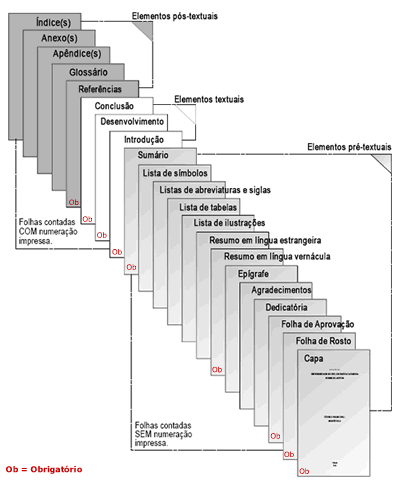
\includegraphics[width=0.6\textwidth]{./04-figuras/abnt}
    \label{fig:ilustfig2}
\end{figure}
\vspace*{-0,9cm}
{\raggedright \fonte{Disponível em: <https://www.intelligentsia.zip.net/estruturamonografia>. Acesso em: 15 ago. 2014.}}\\

Os elementos pré-textuais são compostos de estruturas
obrigatórias: Capa, Folha de ros-to, Folha de aprovação e Sumário. E estruturas opcionais: Lombada, Errata, Dedicatória, Agra-decimentos, Epígrafe, Resumo na língua vernácula, Resumo em língua estrangeira, Lista de ilustrações, Lista de abreviaturas e siglas e Lista de símbolos.

Os elementos textuais são compostos de Introdução,
Desenvolvimento e Conclusão. Os elementos pós-textuais podem é obrigatórios usar as Referências.  E são elementos opcionais: Glossário, Apêndice, Anexo e Índice.

\section{ELEMENTOS PRÉ-TEXTUAIS}

\subsection{Capa}

Elemento obrigatório, sobre o qual se imprimem as informações
indispensáveis à indica-ção do trabalho, na seguinte ordem: nome completo do aluno, título do trabalho, subtítulo se houver, cidade da instituição onde o documento deve ser apresentado, ano de depósito (data da entrega).

\subsection{Lombada}

Elemento opcional, onde as informações devem ser impressas
conforme a norma NBR 12225: nome do autor, impresso longitudinalmente e legível do alto para o pé da lombada. Esta forma possibilita a leitura quando o trabalho está no sentido horizontal, com a face voltada para cima; título do trabalho, impresso da mesma forma que o nome do autor. Elementos alfanuméri-cos de identificação, por exemplo: v. 3.

\subsection{Folha de Rosto}

O anverso da folha de rosto deve conter os elementos na seguinte
ordem: nome completo do aluno, título do trabalho, subtítulo se houver, natureza do trabalho e objetivo (grau pretendi-do), nome da instituição a que é submetido, área de concentração, nome do orientador, local da instituição onde deve ser apresentado, ano de entrega.

\subsection{Errata}

A errata consiste em uma lista das folhas e linhas em que ocorrem
erros, seguida das de-vidas correções. Deve ser inserida após a folha de rosto.

\subsection{Folha de aprovação}

Elemento obrigatório, a folha de aprovação deve conter: nome do
autor, título por exten-so, subtítulo, local e data de aprovação, nome, assinatura e instituição dos membros componen-tes da banca examinadora.

\subsection{Dedicatória}

Folha opcional, onde o aluno presta homenagem ou dedica seu trabalho.

\subsection{Agradecimentos}

Folha opcional, dirigida àqueles que contribuíram para a
elaboração do trabalho.

\subsection{Epígrafe}

Elemento opcional, onde o aluno apresenta uma citação, seguida da
indicação de autoria, relacionada com a matéria tratada no corpo do trabalho. As epígrafes também podem ser apre-sentadas nas folhas de abertura das seções primárias.

\subsection{Resumo}

Consiste na apresentação concisa dos pontos principais de um
texto. Devem ser apresen-tados, de forma clara, os objetivos, o desenvolvimento e as conclusões. Constitui-se em uma sequência de frases objetivas e não uma simples enumeração de tópicos. Deve ser seguido das palavras representativas do conteúdo do trabalho, isto é, palavras-chave e/ou descritores.

\subsection{Abstract}

Consiste em uma versão do resumo em idioma de divulgação
internacional. Deve ser se-guido das palavras representativas do conteúdo do trabalho, isto é, palavras-chave e/ou uniter-mos, na língua.

\subsection{Lista de ilustrações}

As ilustrações (figuras, quadros, tabelas, gráficos) devem ser
numeradas na ordem em que aparecem no texto. É recomendável que sejam feitas listas separadas para cada tipo de ilus-tração. Em cada lista devem constar: número, título e página. Quando as ilustrações forem em grande número e/ou em tamanho maior, podem ser agrupadas no final do trabalho como apên-dice. As ilustrações, com exceção de tabelas, quadros e gráficos, podem ser sinalizadas no texto ou entre parênteses no final da frase, com o termo Figura.

\subsection{Lista de abreviatura e siglas}

Consiste na relação alfabética das abreviaturas e siglas
utilizadas no texto, seguidas das palavras ou expressões correspondentes grafadas por extenso. Recomenda-se a elaboração de lista própria para cada tipo.

\subsection{Lista de símbolos}

Os símbolos devem ser apresentados na lista na ordem em que
aparecem no texto, com o devido significado.

\subsection{Sumário}

Consiste na enumeração das principais divisões, seções e outras
partes do trabalho, na ordem em que aparecem no texto, acompanhadas da página inicial. As divisões devem estar numeradas em algarismos arábicos, a partir da Introdução até às Referências. Havendo subdivi-sões, deve ser adotada a numeração progressiva, sempre em número arábico e a distinção de caracteres, de acordo com a NBR-6027.

\section{ELEMENTOS TEXTUAIS}

\subsection{Introdução}

É a parte inicial do texto onde devem constar a delimitação do
assunto tratado, os objeti-vos da pesquisa e os outros elementos necessários para situar o tema do trabalho.

\subsection{Desenvolvimento}

Parte do texto que contém a exposição ordenada e pormenorizada do
assunto. Divide-se em seções e subseções, que variam em função da abordagem do tema e do método.

\subsection{Conclusão}

Final do texto na qual se apresentam as conclusões correspondentes aos objetivos ou hipóteses.

\section{ELEMENTOS PÓS-TEXTUAIS}

\subsection{Referencias}

É o conjunto padronizado de elementos descritivos, retirados de
um documento, que permite a sua identificação individual. Denomina-se ainda de Referências a lista composta de documentos padronizados e utilizados na elaboração de um trabalho acadêmico.

\subsection{Apêndice}

Consiste em um texto ou um documento elaborado pelo autor, a fim
de complementar sua argumentação, sem prejuízo da unidade nuclear do trabalho. Os apêndices são identificados por letras maiúsculas consecutivas, travessão e pelos respectivos títulos.

\subsection{Anexo}

Consiste em um texto ou documento não elaborado pelo autor, que
serve de fundamen-tação, comprovação e ilustração. Os anexos são identificados por letras maiúsculas consecuti-vas, travessão e pelos respectivos títulos.

\subsection{Índice}

Elemento opcional, elaborado conforme a NBR 6034.

  			% Estrutura    
    %
% Documento: Ilustração
%

\chapter{ILUSTRAÇÕES}

A apresentação de quadros e tabelas está regida pelas Normas de Apresentação Tabular do Instituto Brasileiro de Geografia e Estatística.

\section{FIGURAS}

São desenhos, fotografias, organogramas, esquemas etc. com os respectivos títulos pre-cedidos da palavra Figura e do número de ordem em algarismo arábico.

\begin{figure}[H]
    \centering
    \caption{Exemplo de figura}
	\vspace*{0,2cm}
    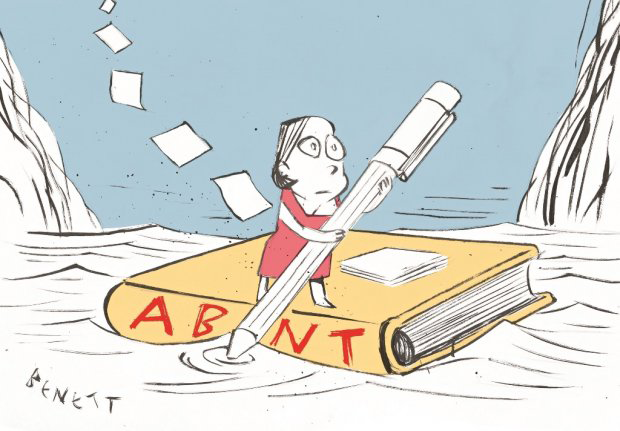
\includegraphics[width=0.8\textwidth]{./04-figuras/navegar_abnt}
    \label{fig:ilustfig}
\end{figure}
\vspace*{-0,9cm}
{\raggedright \fonte{Disponível em: <https://www.gazetadopovo.com.br/abntemfoco>. Acesso em: 24 de jan. de 2015.}}\\

Os títulos devem ser colocados acima das figuras. No texto devem
ser indicados pela pa-lavra Figura acompanhada do número de ordem. E abaixo deve ser indicada sua fonte.

\section{QUADROS}

Denomina-se quadro a apresentação de dados de forma organizada, para cuja compreen-são não seria necessário qualquer elaboração matemático-estatística. A identificação se fará com o nome do elemento Quadro por extenso, seguido do número de ordem em algarismo arábico. Outros elementos do quadro deverão ser descritos de acordo com o padrão usado para
Apresentação tabular.

\begin{quadro}[H]

	\begin{center}
	\caption{Exemplo para quadro.\label{qua:quaexe}}
		\begin{tabular}{|p{7cm}|p{7cm}|}
			\hline
			("Trabalho Conclusão de Curso")\\
			\hline
			
		\end{tabular}
	\end{center}
	\vspace*{-0,8cm}

	{\raggedright \fonte{Autor desta monografia, 2015.}}
	
\end{quadro}




\section{TABELAS}

Tabelas são conjuntos de dados numéricos, associados a um
fenômeno, dispostos numa determinada ordem da classificação. Expressam as variações qualitativas e quantitativas de um fenômeno. A finalidade básica da tabela é resumir ou sintetizar dados de maneira a fornecer o máximo de informações num mínimo de espaço.

Na apresentação de uma tabela devem ser levados em consideração
os alguns critérios. Toda tabela deve ter significado próprio, dispensando consultas ao texto. A tabela deve ser colo-cada em posição vertical, para facilitar a leitura dos dados. No caso em que isso seja impossível, deve ser colocada em posição horizontal, com o título voltado para a margem esquerda da folha.

Se a tabela ou quadro não couber em uma página, deve ser
continuado na página seguin-te. Neste caso o final não será delimitado por traço horizontal na parte inferior e o cabeçalho será repetido na página seguinte. No texto devem ser indicadas pela palavra Tabela acompanha-da do número de ordem em algarismo arábico.

\begin{table}[H]
    \centering
    \caption[Exemplo tabela]{Exemplo tabela.\label{tab:exetab}}
    \begin{tabular}{cc}
        \hline
            numeros x & numeros y \\
        \hline
            \vspace*{0,15cm} 1 & 15 \vspace*{0,15cm}\\ \hline
            \vspace*{0,15cm} 3 & 4 \vspace*{0,15cm}\\ \hline
            \vspace*{0,15cm} 5 & 6 \vspace*{0,15cm}\\ \hline
            \vspace*{0,15cm} 7 & 8 \vspace*{0,15cm}\\ \hline
			\vspace*{0,15cm} 9 & 11 \vspace*{0,15cm}\\ \hline
            \vspace*{0,15cm} 13 & 15 \vspace*{0,15cm}\\ \hline
        \hline
    \end{tabular}
\end{table}
\vspace*{-0,9cm}
{\raggedright \fonte{Autor desta monografia, 2014.}}





\section{GRÁFICOS}

Depois de sintetizados em tabelas, os dados podem ser
apresentados em gráficos, com a fi-nalidade de proporcionar ao interessado uma visão rápida do comportamento do fenômeno. Serve para representar qualquer tabela de maneira simples, legível e interessante, tornando cla-ros os fatos que poderiam passar despercebidos em dados apenas tabulados.

O elemento de identificação ordenado do gráfico, ou seja, o
número de ordem do mesmo no trabalho. No texto devem ser indicados pela palavra Gráfico, acompanhada do número de ordem em algarismo arábico.



           	% Ilustrações
    %
% Documento: Citações
%

\chapter{CITAÇÕES}

Citação é a menção, no texto, de uma informação colhida de outra fonte. Pode ser direta, indireta e citação de citação. Apresentadas conforme a ABNT NBR 10520

\section{CITAÇÃO DIRETA}

É a transcrição textual dos conceitos de um autor consultado. Um
exemplo: De acordo com as conclusões de Marshall (1980, p. 249) “da mesma forma que não se pode afirmar se é a lâmina inferior ou superior de uma tesoura que corta uma folha de papel, também não se pode discutir se o valor e os preços são governados pela utilidade ou pelo custo de produção”. 

Citação mais longa deve figurar abaixo do texto, em bloco recuado
– de 4 cm da mar-gem esquerda – com letras tamanho 10, sem aspas.

\section{CITAÇÃO INDIRETA}

É a transcrição livre do texto do autor consultado. As citações
indiretas ou parafraseadas dispensam o uso de aspas duplas e do número de páginas.

A produção acadêmica sobre varejo no Brasil fica muito aquem da
importância do seg-mento na economia (ANGELO; SILVA, 1993). É um exemplo de citação indireta.

\section{CITAÇÃO DE CITAÇÃO}

É citação direta ou indireta de um documento ao qual não se teve
acesso aooriginal. De-ve ser citado em nota de rodapé, sendo obrigatória a indicação da Fonte 10 recuo de 4 cm refe-rência de onde foi extraída a informação. Esse tipo de citação só deve ser utilizado nos casos em que realmente o documento original não pode ser recuperado. 

Exemplo: Enguita (apud SILVA, 1991, p. 21) chegou às mesmas
conclusões. As entida-des coletivas podem ser citadas pelas respectivas siglas, desde que na primeira vez em que fo-rem mencionadas apareçam por extenso. Exemplo: ASSOCIAÇÃO BRASILEIRA DO TRA-BALHADOR - ABT (1985)


            	% Citações
    %
% Documento: Tecnicas de referencia
%

\chapter{TÉCNICAS DE REFERÊNCIAS}

É o conjunto padronizado de elementos descritivos, retirados de um documento, que permite a sua identificação individual. Denomina-se ainda de Referências a lista composta de documentos padronizados e utilizados na elaboração de um trabalho acadêmico.

O texto deve estar com o alinhamento justificado, respeitando a formatação indicada pa-ra o tipo de referência. 

\section{MONOGRAFIA}

Monografia Considerada no Todo (livros, folhetos, dissertações,
teses, dicionários, guias). Exemplos: <SOBRENOME, Nome do Autor>. \textbf{Nome
da obra.} Edição.

\section{LIVROS TENDO A ENTIDADE COMO AUTOR}

<NOME DA ENTIDADE>. \textbf{Nome do livro.} Edição.

\section{DOCUMENTOS ELABORADOS POR VÁRIOS AUTORES}

Documentos elaborados por vários autores, com um responsável
intelectual destacado (organizador, coordenador, editor). Exemplo: <SOBRENOME,
Nome do Autor> (Responsabi-lidade atribuída). \textbf{Nome da obra.} Edição.

\section{DOCUMENTOS SEM AUTOR}

<DOCUMENTO e seus subtítulo, caso exista>. Edição. 

\section{ARTIGO OU MATERIA DE REVISTA}

<SOBRENOME, Nome do Autor>. Titulo da matéria. \textbf{Nome da
revista.} Edição.

\section{DOCUMENTO DE EVENTO}

<NOME DO EVENTO, data e local>. Organizador do Evento. Ano,
pagina dos anais onde se encontra a obra. 

\section{EXEMPLOS PARA CITAÇÕES}

Apenas exemplos \cite{7.1.3-1}. Outro \cite{NBR6023:2000}.\cite{NBR10520:1988}. \cite{7.3.2-2}. \cite{7.4.2.1-3}. \cite{7.4.2.1-2}.\cite{7.4.2.3-5}. \cite{7.4.2.1-4}. 
\cite{7.7.1.2-5}. \cite{7.7.1.2-2}. \cite{7.4.2.3-6}. \cite{8.1.1.5}.
            % Tecnica de referencias 

    % Elementos pós textuais
    \postextual
    %
% Documento: Referências Bibliográficas
%

\bibliography{refrtf}    % Geração automática das referências por meio do arquivo 'refbase.bib'
       % Referências
    %
% Documento: Apêndices
%

\begin{apendicesenv}

\chapter{Como elaborar}

Apêndice é texto ou documento elaborado pelo autor, a fim de
complementar sua argu-mentação, sem prejuízo da unidade nuclear do trabalho. Documentos elaborados por vários au-tores, com um responsável intelectual destacado (organizador, coordenador Elemento opcional.  Deve ser precedido da palavra APÊNDICE, identificado por letras maiúsculas consecutivas, travessão e pelo respectivo título. Utilizam-se letras maiúsculas dobradas, na identificação dos apêndices, quando esgotadas as letras do alfabeto.

\end{apendicesenv}
         % Apêndices
    %
% Documento: Anexos
%

\begin{anexosenv}

\chapter{Como elaborar}

Anexo é texto ou documento não elaborado pelo autor, que serve de fundamentação, comprovação e ilustração. Elemento opcional. Deve ser precedido da palavra ANEXO, identifi-cado por letras maiúsculas consecutivas, travessão e pelo respectivo título. Utilizam-se letras maiúsculas dobradas, na identificação dos anexos, quando esgotadas as letras do alfabeto.


\end{anexosenv}            % Anexos
    %\printindex                                             % Índice remissivo

\end{document}
